\section{Berbagai macam Jenis Sensor}
\section{Pengertian Sensor Suara}
Sensor suara merupakan sensor yang mensensing besaran suara untuk diubah menjadi besaran listrik. Sensor ini bekerja berdasarkan besar kecilnya kekuatan gelombang suara yang diterima. Dimana gelombang suara tersebut mengenai membran sensor, yang menyebabkan bergeraknya membran sensor yang memiliki kumparan kecil sehingga menghasilkan besaran listrik. Kecepatan bergeraknya kumparan kecil tersebut menentukan kuat lemahnya gelombang listrik yang akan dihasilkan. Salah satu contoh komponen yang termasuk dalam sensor ini adalah condeser microphone atau mic. Bentuk fisik dari condeser mic yaitu berbentuk bulat dan memiliki kaki dua seperti contoh pada gambar \ref{fig:sscondesermic}.
\begin{figure}[!htbp]
  \centering
  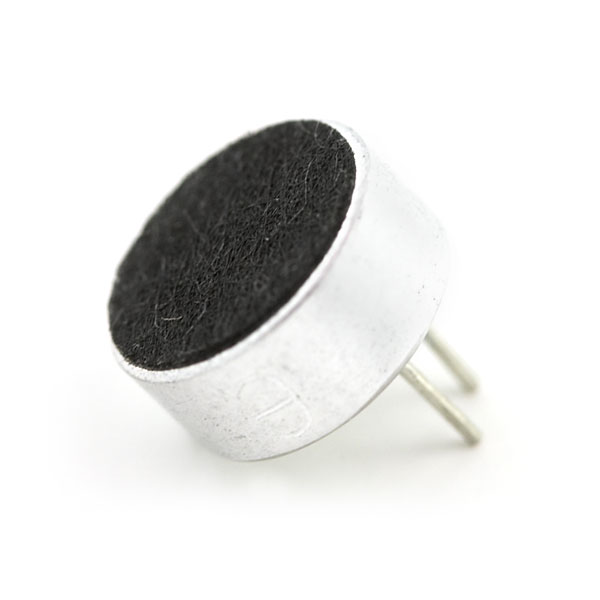
\includegraphics[width=.75\textwidth]{figures/Arduino/sscondesermic.jpg}
  \caption{Ini adalah Condeser Microphone}\label{fig:sscondesermic}
\end{figure}

\subsection{Prinsip Kerja Condeser Microphone}
Condenser mic biasanya bekerja berdasarkan susunan backplate atau diafragma yang harus terhubung dengan listrik dan membentuk kapasitor sound - sensitive. Gelombang suara yang tercipta akan masuk ke microphone dan akan menggetarkan komponen diafragma ini. Letak dari diafragma ditempatkan di depan sebuah backplate. Susunan dari elemen - elemen tersebut akan membentuk sebuah kapasitor yang sering disebut juga sebagai kondenser. Kapasitor memiliki kemampuan untuk menyimpan muatan maupun tegangan. Ketika elemen tersebut terisi dengan muatan, medan listrik akan terbentuk di antara diafragma dan backplate, yang dimana besarnya itu proporsional terhadap ruang yang terbentuk diantaranya. Macam - macam lebar dari jarak antara backplate dengan diafragma yang terjadi disebabkan karena adanya pergerakan oleh diafragma relatif terhadap backplate yang dikarenakan adanya tekanan suara yang mengenai diafragma. Hal ini akan menghasilkan sinyal elektrik dari gelombang suara yang masuk ke condenser microphone seperti contoh pada gambar \ref{fig:sscondesermicscheme}.
\begin{figure}[!htbp]
  \centering
  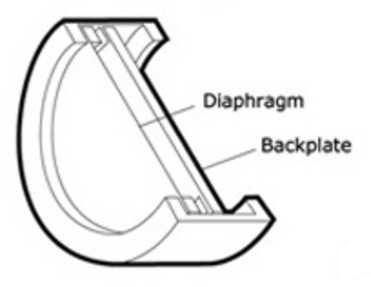
\includegraphics[width=.75\textwidth]{figures/Arduino/sscondesermicscheme.jpg}
  \caption{Ini adalah Skema dari Condeser Microphone}\label{fig:sscondesermicscheme}
\end{figure}

\subsection{Karakteristik dari Condeser Microphone}

Karakteristik dari Conseder Microphone adalah sebagai berikut :

\begin{enumerate}
  \item Susunannya lebih kompleks dibanding dengan jenis microphone lainnya seperti dibanding dengan dynamic Microphone.
  \item Pada frekuensi tinggi, akan menghasilkan suara yang lebih halus dan natural, serta sensitivitas yang lebih tinggi.
  \item Mudah akan mencapai respon frekuensi flat dan memiliki range frekuensi yang lebih luas.
  \item Ukurannya lebih kecil dibanding dengan jenis tipe mikrophone lainnya.
\end{enumerate}

Pada pasaran sudah dijual sensor suara menggunakan condeser mic ini dalam bentuk modul, sehingga mudah dan praktis dalam penggunaannya.

\begin{figure}[!htbp]
  \centering
  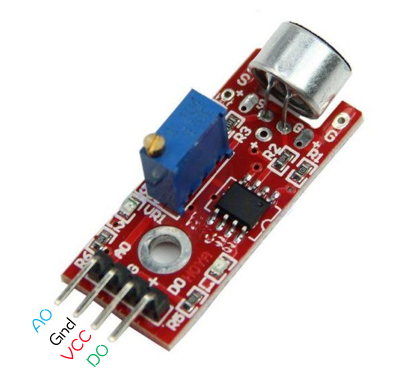
\includegraphics[width=.75\textwidth]{figures/Arduino/sssensorsuara.png}
  \caption{Ini adalah Skema dari Condeser Microphone}\label{fig:sssensorsuara}
\end{figure}	

Spesifikasi dari modul sensor suara seperti contoh pada gambar \ref{fig:sssensorsuara} adalah sebagai berikut :

\begin{enumerate}
  \item Sensitivitas dapat diatur (pengaturan manual pada potensiometer).
  \item Condeser yang digunakan memiliki sensitivitas yang tinggi.
  \item Tegangan kerja antara 3.3V – 5V.
  \item Terdapat 2 pin keluaran yaitu tegangan analog dan digital output.
  \item Sudah terdapat lubang baut untuk instalasi.
  \item Sudah terdapat indikator led.
\end{enumerate} 

\section{Sensor Gas}
\begin{figure}[!htbp]
  \centering
  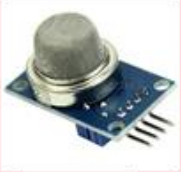
\includegraphics[width=.75\textwidth]{figures/mq2.png}
  \caption{Ini adalah Sensor suhu MQ-2 \cite{himawan2017perancangan}}\label{fig:mq2}
\end{figure}	
Sensor yang digunakan kali ini adalah sensor MQ-2 seperti pada gambar \ref{fig:mq2}, sensor ini digunakan untuk mendeteksi gas LPG, i-butana, propana, alkohol, hidroge, dan asap. Inti dari MQ-2 adalah material yang sensitif terhadap konsentrasi gas yang tersusun dari senyawa SnO2 atau Timah Oksida. Material ini mempunyai karakteristik yang akan merubah konduktivitasnya seiring dengan perubahan konsenterasi gas.
Seri MQ sensor gas menggunakan pemanas kecil di dalamnya dengan sensor elektro-kimia. Mereka sensitif terhadap berbagai gas dan digunakan di dalam ruangan pada suhu kamar.
Mereka dapat dikalibrasi lebih atau kurang lihat bagian tentang Load-resistor dan Burn-in namun diketahui konsentrasi gas atau gas yang diukur diperlukan untuk itu.
Outputnya adalah sinyal analog dan bisa dibaca dengan input analog Arduino.
Sedangkan untuk spesifikasi sensor MQ-2, adalah:
\begin{itemize}
\item suhu 20 derajat Celcius
\item kelembaban udara 65 persen
\end{itemize}
range konsentrasi gas yang bisa diukur:
\begin{itemize}
\item LPG dan propana: 200ppm-5000ppm
\item butana: 300ppm-5000ppm
\item metana: 5000ppm - 20000ppm
\end{itemize}

\section{Sensor Infrared}
\subsection{Infrared Obstacle Detector}
\begin{figure}[!htbp]
  \centering
  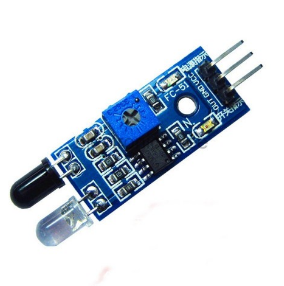
\includegraphics[width=.75\textwidth]{figures/Arduino/sensorinfrared.png}
  \caption{Ini adalah Sensor Infrared Obstacle Detector}\label{fig:obstacle}
\end{figure}
Sensor infrared obstacle detector seperti pada gambar \ref{fig:obstacle} memanfaatkan kondisi apabila infrared pada sensor ditutup maka LED notifikasi akan menyala, sensor ini bekerja dengan memanfaatkan infrared, apabila cahaya infrared diterima dengan cahaya yang cukup terang maka lampu tidak menyala dan apabila cahaya infrared diterima dengan pencerahan cahaya yang kurang maka lampu akan menyala sebagai pengganti penerangan. Kegunaan dari Infrared Obstacle Detector digunakan untuk mendeteksi penerangan cahaya dengan memanfaatkan sinar infrared yang ada pada sensor tersebut. Cara kerja dari Infrared Obstacle Detector yaitu apabila ada penghalang yang menghalangi sinar infrared maka LED notifikasi akan menyala.

\section{Sensor Cahaya}
\begin{figure}[!htbp]
  \centering
  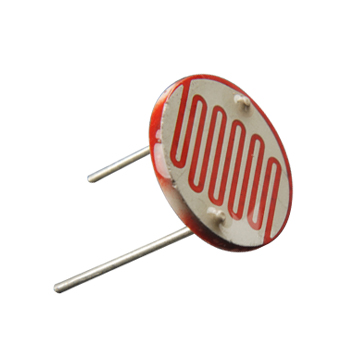
\includegraphics[width=.75\textwidth]{figures/Arduino/LDR.jpg}
  \caption{Ini adalah Sensor LDR}\label{fig:ldr}
\end{figure}

\subsection{Pengertian}
Sensor cahaya atau LDR merupakan sensor yang di pakai untuk mengubah besaran listrik menjadi besaran cahaya atau pengertian lain adalah  sensor yang membuat kita dapat melakukan pendeteksian cahaya, dan melakukan perubahan terhadap cahaya tersebut ,jadi sinyal listrik dan dipakai dalam sebuah rangkaian yang menggunakan cahaya sebagai alat pemicunya. Prinsip-prinsip kerja dari alat tersebut adalah untuk mengubah suatu energi dari foton menjadi elektron. Idealnya satu foton dapat membangkitkan satu elektron. Sensor cahaya sangat banyak penggunaannya, salah satu yang paling populer adalah kamera digital. Pada saat ini sudah ada alat yang digunakan untuk mengukur cahaya yang mempunyai 1 buah foton saja.

\subsection{Karakteristik Sensor}
Sensor Cahaya LDR (Light Dependent Resistor) merupakan suatu bentuk komponen yang mempunyai perubahan resistansi yang besarnya tergantung pada cahaya. Karakteristik LDR terdiri dari dua macam yaitu yang pertama Laju Recovery dan Respon Spektral.

Karakteristik sensor LDR adalah sebagai berikut :

\begin{itemize}
	\item LDR tipe arus harganya lebih besar dari 200K/detik.
	\item tidak mempunyai sensitivitas yang sama untuk setiap panjang gelombang cahaya yang jatuh padanya (yaitu warna).
	\item Dalam keadaan gelap resistansi LDR seki-tar 10MΩ dan dalam keadaan terang sebe-sar 1KΩ atau kurang.
\end{itemize}


